% Options for packages loaded elsewhere
\PassOptionsToPackage{unicode}{hyperref}
\PassOptionsToPackage{hyphens}{url}
%
\documentclass[
]{article}
\usepackage{amsmath,amssymb}
\usepackage{lmodern}
\usepackage{iftex}
\ifPDFTeX
  \usepackage[T1]{fontenc}
  \usepackage[utf8]{inputenc}
  \usepackage{textcomp} % provide euro and other symbols
\else % if luatex or xetex
  \usepackage{unicode-math}
  \defaultfontfeatures{Scale=MatchLowercase}
  \defaultfontfeatures[\rmfamily]{Ligatures=TeX,Scale=1}
\fi
% Use upquote if available, for straight quotes in verbatim environments
\IfFileExists{upquote.sty}{\usepackage{upquote}}{}
\IfFileExists{microtype.sty}{% use microtype if available
  \usepackage[]{microtype}
  \UseMicrotypeSet[protrusion]{basicmath} % disable protrusion for tt fonts
}{}
\makeatletter
\@ifundefined{KOMAClassName}{% if non-KOMA class
  \IfFileExists{parskip.sty}{%
    \usepackage{parskip}
  }{% else
    \setlength{\parindent}{0pt}
    \setlength{\parskip}{6pt plus 2pt minus 1pt}}
}{% if KOMA class
  \KOMAoptions{parskip=half}}
\makeatother
\usepackage{xcolor}
\usepackage[margin=1in]{geometry}
\usepackage{graphicx}
\makeatletter
\def\maxwidth{\ifdim\Gin@nat@width>\linewidth\linewidth\else\Gin@nat@width\fi}
\def\maxheight{\ifdim\Gin@nat@height>\textheight\textheight\else\Gin@nat@height\fi}
\makeatother
% Scale images if necessary, so that they will not overflow the page
% margins by default, and it is still possible to overwrite the defaults
% using explicit options in \includegraphics[width, height, ...]{}
\setkeys{Gin}{width=\maxwidth,height=\maxheight,keepaspectratio}
% Set default figure placement to htbp
\makeatletter
\def\fps@figure{htbp}
\makeatother
\setlength{\emergencystretch}{3em} % prevent overfull lines
\providecommand{\tightlist}{%
  \setlength{\itemsep}{0pt}\setlength{\parskip}{0pt}}
\setcounter{secnumdepth}{-\maxdimen} % remove section numbering
\usepackage{booktabs}
\usepackage{longtable}
\usepackage{array}
\usepackage{multirow}
\usepackage{wrapfig}
\usepackage{float}
\usepackage{colortbl}
\usepackage{pdflscape}
\usepackage{tabu}
\usepackage{threeparttable}
\usepackage{threeparttablex}
\usepackage[normalem]{ulem}
\usepackage{makecell}
\usepackage{xcolor}
\ifLuaTeX
  \usepackage{selnolig}  % disable illegal ligatures
\fi
\IfFileExists{bookmark.sty}{\usepackage{bookmark}}{\usepackage{hyperref}}
\IfFileExists{xurl.sty}{\usepackage{xurl}}{} % add URL line breaks if available
\urlstyle{same} % disable monospaced font for URLs
\hypersetup{
  pdftitle={Analysis of the 12 journal LDA},
  pdfauthor={Brian Weatherson},
  hidelinks,
  pdfcreator={LaTeX via pandoc}}

\title{Analysis of the 12 journal LDA}
\author{Brian Weatherson}
\date{}

\begin{document}
\maketitle

\hypertarget{keywords-for-all-topics}{%
\subsection{Keywords for All Topics}\label{keywords-for-all-topics}}

\begin{tabular}{rl}
\toprule
1 & bradleys, bradley, schiller, jamess, pragmatist\\
2 & psychic, introspective, neural, inorganic, mechanistic\\
3 & cent, painting, average, esthetic, random\\
4 & neururgic, circuit, noetic, educational, sec\\
5 & motor, responses, reflex, affective, sensory\\
6 & apprehended, spatial, colour, temporal, stout\\
7 & design, behaviour, horse, predict, springs\\
8 & hegels, bosanquet, hegel, hegelian, phenomenal\\
9 & institutions, social, economic, ethical, happiness\\
10 & instrumental, dewey, deweys, reflective, relationships\\
11 & lovejoy, realists, perry, realist, realistic\\
12 & sensedata, lockes, perceiving, locke, acquaintance\\
13 & judg, judgments, beliefs, judgment, judging\\
14 & western, cultural, philosophies, santayana, philoso\\
15 & medical, mystic, novelty, aesthetic, miss\\
16 & quod, augustine, schopenhauer, esse, sit\\
17 & velocity, spacetime, equations, physicists, measurement\\
18 & deductive, inductive, syllogism, mathematicians, logicians\\
19 & propositional, proposi, entails, principia, propositions\\
20 & france, paris, french, paul, devoted\\
21 & spinozas, spinoza, cartesian, descartes, leibniz\\
22 & rep, platos, parmenides, plato, platonic\\
23 & legal, morally, rights, pity, prima\\
24 & husserl, humes, berkeleys, kants, edition\\
25 & linguistic, fears, sentences, grammatical, meaningful\\
\bottomrule
\end{tabular}
\newpage

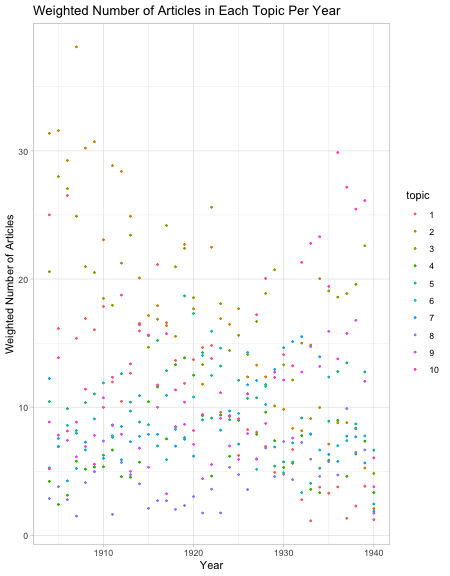
\includegraphics{early-lda-summary_files/figure-latex/weight-1.pdf}
\newpage 
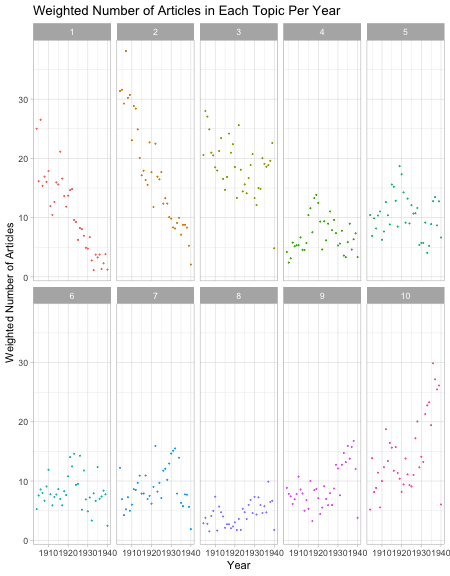
\includegraphics{early-lda-summary_files/figure-latex/weight-2.pdf}
\newpage 

\hypertarget{topic-1}{%
\subsection{Topic 1}\label{topic-1}}

\textbf{Keywords}: bradleys, bradley, schiller, jamess, pragmatist,
bosanquet, pragmatism, pragmatists, pragmatic, james, condemned,
scepticism, coherence, taylor, recognise

\includegraphics{early-lda-summary_files/figure-latex/cats-1.pdf}
\newpage 

\hypertarget{characteristic-articles-for-topic-1}{%
\subsubsection{Characteristic Articles for Topic
1}\label{characteristic-articles-for-topic-1}}

\begin{enumerate}
\def\labelenumi{\arabic{enumi}.}
\item
  F. H. Bradley, 1907, ``On Truth and Copying,'' \emph{Mind}
  16:165--180.
\item
  F. H. Bradley, 1910, ``On Appearance, Error and Contradiction,''
  \emph{Mind} 19:153--185.
\item
  F. H. Bradley, 1911, ``On Some Aspects of Truth,'' \emph{Mind}
  20:305--341.
\item
  F. C. S. Schiller, 1910, ``The Present Phase of `Idealist'
  Philosophy,'' \emph{Mind} 19:30--45.
\item
  F. C. S. Schiller, 1915, ``The New Developments of Mr.~Bradley's
  Philosophy,'' \emph{Mind} 24:345--366.
\item
  F. H. Bradley, 1909, ``Coherence and Contradiction,'' \emph{Mind}
  18:489--508.
\item
  F. H. Bradley, 1904, ``On Truth and Practice,'' \emph{Mind}
  13:309--335.
\item
  F. C. S. Schiller, 1904, ``In Defence of Humanism,'' \emph{Mind}
  13:525--542.
\item
  F. C. S. Schiller, 1907, ``Mr.~Bradley's Theory of Truth,''
  \emph{Mind} 16:401--409.
\item
  F. C. S. Schiller, 1910, ``Absolutism in Extremis?,'' \emph{Mind}
  19:533--540.
\item
  F. C. S. Schiller, 1908, ``Is Mr.~Bradley Becoming a Pragmatist?,''
  \emph{Mind} 17:370--383.
\item
  F. C. S. Schiller, 1913, ``Mysticism v. Intellectualism,'' \emph{Mind}
  22:87--89.
\item
  R. F. Alfred Hoernle, 1905, ``Pragmatism v. Absolutism (I.),''
  \emph{Mind} 14:297--334.
\item
  Douglas Fawcett, 1918, ``Some Observations Touching the Cosmic
  Imagining and''Reason'','' \emph{Mind} 27:152--164.
\item
  F. C. S. Schiller, 1922, ``An Idealist in Extremis,'' \emph{Mind}
  31:144--153.
\end{enumerate}

\newpage

\hypertarget{topic-2}{%
\subsection{Topic 2}\label{topic-2}}

\textbf{Keywords}: psychic, introspective, neural, inorganic,
mechanistic, psychophysical, psychologist, biological, evolutionary,
introspection, psy, chology, nervous, physiological, biology

\includegraphics{early-lda-summary_files/figure-latex/cats-2.pdf}
\newpage 

\hypertarget{characteristic-articles-for-topic-2}{%
\subsubsection{Characteristic Articles for Topic
2}\label{characteristic-articles-for-topic-2}}

\begin{enumerate}
\def\labelenumi{\arabic{enumi}.}
\item
  Mary Whiton Calkins, 1908, ``Psychology as Science of Self: I. Is the
  Self Body or Has it Body?,'' \emph{The Journal of Philosophy,
  Psychology and Scientific Methods} 5:12--20.
\item
  Henry Rutgers Marshall, 1904, ``Of Simpler and More Complex
  Consciousnesses,'' \emph{The Journal of Philosophy, Psychology and
  Scientific Methods} 1:365--372.
\item
  Howard C. Warren, 1916, ``A Study of Purpose. II Purposive Activity in
  Organisms,'' \emph{The Journal of Philosophy, Psychology and
  Scientific Methods} 13:29--49.
\item
  Charles H. Judd, 1908, ``The Doctrine of Attitudes,'' \emph{The
  Journal of Philosophy, Psychology and Scientific Methods} 5:676--684.
\item
  Henry Rutgers Marshall, 1904, ``Of Neururgic and Noetic
  Correspondences,'' \emph{The Journal of Philosophy, Psychology and
  Scientific Methods} 1:309--316.
\item
  Howard C. Warren, 1918, ``Mechanism Versus Vitalism, in the Domain of
  Psychology,'' \emph{The Philosophical Review} 27:597--615.
\item
  Mary Whiton Calkins, 1907, ``Psychology: What is it About?,''
  \emph{The Journal of Philosophy, Psychology and Scientific Methods}
  4:673--683.
\item
  A. P. Weiss, 1919, ``The Relation Between Physiological Psychology and
  Behavior Psychology,'' \emph{The Journal of Philosophy, Psychology and
  Scientific Methods} 16:626--634.
\item
  Mary Whiton Calkins, 1917, ``Purposing Self Versus Potent Soul: A
  Discussion of Professor Warren's''Study of Purpose'','' \emph{The
  Journal of Philosophy, Psychology and Scientific Methods} 14:197--200.
\item
  Arthur F. Bentley, 1939, ``Situational Treatments of Behavior,''
  \emph{The Journal of Philosophy} 36:309--323.
\item
  Charles Hughes Johnston, 1907, ``Feeling Analysis and
  Experimentation,'' \emph{The Journal of Philosophy, Psychology and
  Scientific Methods} 4:209--215.
\item
  Mary Whiton Calkins, 1908, ``Psychology as Science of Self: III. The
  Description of Consciousness,'' \emph{The Journal of Philosophy,
  Psychology and Scientific Methods} 5:113--122.
\item
  Robert M. Yerkes, 1905, ``Animal Psychology and Criteria of the
  Psychic,'' \emph{The Journal of Philosophy, Psychology and Scientific
  Methods} 2:141--149.
\item
  Grace A. de Laguna, 1919, ````Dualism and Animal Psychology:'' A
  Rejoinder,'' \emph{The Journal of Philosophy, Psychology and
  Scientific Methods} 16:296--300.
\item
  Ralph S. Lillie, 1926, ``The Nature of the Vitalistic Dilemma,''
  \emph{The Journal of Philosophy} 23:673--682.
\end{enumerate}

\newpage

\hypertarget{topic-3}{%
\subsection{Topic 3}\label{topic-3}}

\textbf{Keywords}: cent, painting, average, esthetic, random, table,
records, colors, six, musical, pictures, angle, eye, twice, visual

\includegraphics{early-lda-summary_files/figure-latex/cats-3.pdf}
\newpage 

\hypertarget{characteristic-articles-for-topic-3}{%
\subsubsection{Characteristic Articles for Topic
3}\label{characteristic-articles-for-topic-3}}

\begin{enumerate}
\def\labelenumi{\arabic{enumi}.}
\item
  Henry F. Adams, 1915, ``The Relative Importance of Size and Frequency
  in Forming Associations,'' \emph{The Journal of Philosophy, Psychology
  and Scientific Methods} 12:477--491.
\item
  Henry F. Adams, 1916, ``The Relative Memory Values of Duplication and
  Variation in Advertising,'' \emph{The Journal of Philosophy,
  Psychology and Scientific Methods} 13:141--152.
\item
  June E. Downey, 1914, ``Judgments on Handwriting Similarity and
  Difference,'' \emph{The Journal of Philosophy, Psychology and
  Scientific Methods} 11:544--553.
\item
  George F. Williamson, 1915, ``Individual Differences in Belief,
  Measured and Expressed by Degrees of Confidence,'' \emph{The Journal
  of Philosophy, Psychology and Scientific Methods} 12:127--137.
\item
  E. K. Strong, Jr., 1911, ``Application of the''Order of Merit Method''
  to Advertising,'' \emph{The Journal of Philosophy, Psychology and
  Scientific Methods} 8:600--606.
\item
  Shepherd Ivory Franz, 1905, ``The Reeducation of an Aphasic,''
  \emph{The Journal of Philosophy, Psychology and Scientific Methods}
  2:589--597.
\item
  Edward K. Strong, Jr., 1914, ``Two Factors which Influence Economical
  Learning,'' \emph{The Journal of Philosophy, Psychology and Scientific
  Methods} 11:124--131.
\item
  Kate Gordon, 1915, ``A Study of an Imagery Test,'' \emph{The Journal
  of Philosophy, Psychology and Scientific Methods} 12:574--579.
\item
  June E. Downey, 1912, ``Literary Synesthesia,'' \emph{The Journal of
  Philosophy, Psychology and Scientific Methods} 9:490--498.
\item
  E. L. Thorndike, 1916, ``The Technique of Combining Incomplete
  Judgments of the Relative Positions of N Facts made by N Judges,''
  \emph{The Journal of Philosophy, Psychology and Scientific Methods}
  13:197--204.
\item
  T. K. Abbott, 1904, ``Fresh Light on Molyneux' Problem. Dr.~Ramsay's
  Case,'' \emph{Mind} 13:543--554.
\item
  Edith F. Mulhall, 1914, ``Experiments in Judgment,'' \emph{The Journal
  of Philosophy, Psychology and Scientific Methods} 11:577--583.
\item
  Margaret Hart Strong; H. L. Hollingworth, 1912, ``The Influence of
  Form and Category on the Outcome of Judgment,'' \emph{The Journal of
  Philosophy, Psychology and Scientific Methods} 9:513--520.
\item
  Garry C. Myers, 1915, ``Affective Factors in Recall,'' \emph{The
  Journal of Philosophy, Psychology and Scientific Methods} 12:85--92.
\item
  T. K. Slade, 1925, ``An Enquiry Into the Nature of Colour
  Associations,'' \emph{Mind} 34:455--470.
\end{enumerate}

\newpage

\hypertarget{topic-4}{%
\subsection{Topic 4}\label{topic-4}}

\textbf{Keywords}: neururgic, circuit, noetic, educational, sec,
electric, statistical, display, henry, tests, teachers, imagery, minor,
laboratory, testing

\includegraphics{early-lda-summary_files/figure-latex/cats-4.pdf}
\newpage 

\hypertarget{characteristic-articles-for-topic-4}{%
\subsubsection{Characteristic Articles for Topic
4}\label{characteristic-articles-for-topic-4}}

\begin{enumerate}
\def\labelenumi{\arabic{enumi}.}
\item
  W. H. Winch, 1911, ``The Faculty Doctrine, Correlation, and
  Educational Theory. II,'' \emph{The Journal of Philosophy, Psychology
  and Scientific Methods} 8:372--384.
\item
  Sherwin Cody, 1920, ``Enlarging the Scope of Mental Measurement,''
  \emph{The Journal of Philosophy, Psychology and Scientific Methods}
  17:572--579.
\item
  H. L. Hollingworth, 1910, ``The Central Tendency of Judgment,''
  \emph{The Journal of Philosophy, Psychology and Scientific Methods}
  7:461--469.
\item
  Linius W. Kline, 1914, ``An Experimental Study for Classes in
  Reasoning and its Transference,'' \emph{The Journal of Philosophy,
  Psychology and Scientific Methods} 11:633--638.
\item
  W. H. Winch, 1910, ``\,`Physiological' and `Psychological',''
  \emph{Mind} 19:200--217.
\item
  Beardsley Ruml, 1917, ``Coefficients of Diagnostic Value,'' \emph{The
  Journal of Philosophy, Psychology and Scientific Methods} 14:633--637.
\item
  R. M. Ogden, 1913, ``Content versus''Kundgabe'' in Introspection,''
  \emph{The Journal of Philosophy, Psychology and Scientific Methods}
  10:403--411.
\item
  E. A. Singer, Jr., 1929, ``On the Conscious Mind,'' \emph{The Journal
  of Philosophy} 26:561--575.
\item
  Beardsley Ruml, 1921, ``Reconstruction in Mental Tests,'' \emph{The
  Journal of Philosophy} 18:181--185.
\item
  Frances H. Rousmaniere, 1909, ``The Bases for Generalization in
  Scientific Methods,'' \emph{The Journal of Philosophy, Psychology and
  Scientific Methods} 6:202--205.
\item
  W. H. Winch, 1909, ``A Modern Basis for Educational Theory,''
  \emph{Mind} 18:84--104.
\item
  Frederic Lyman Wells, 1906, ``Linguistic Standards,'' \emph{The
  Journal of Philosophy, Psychology and Scientific Methods} 3:431--435.
\item
  A. T. Poffenberger, 1922, ``Measures of Intelligence and Character,''
  \emph{The Journal of Philosophy} 19:261--266.
\item
  Gregory H. S. Razran, 1935, ``Psychology in the U. S. S. R,''
  \emph{The Journal of Philosophy} 32:19--24.
\item
  Margaret Floy Washburn, 1917, ``Some Thoughts on the Last Quarter
  Century in Psychology,'' \emph{The Philosophical Review} 26:46--55.
\end{enumerate}

\newpage

\hypertarget{topic-5}{%
\subsection{Topic 5}\label{topic-5}}

\textbf{Keywords}: motor, responses, reflex, affective, sensory,
stimulation, stimuli, cerebral, nerve, stimulus, muscular, neural,
nervous, response, aroused

\includegraphics{early-lda-summary_files/figure-latex/cats-5.pdf}
\newpage 

\hypertarget{characteristic-articles-for-topic-5}{%
\subsubsection{Characteristic Articles for Topic
5}\label{characteristic-articles-for-topic-5}}

\begin{enumerate}
\def\labelenumi{\arabic{enumi}.}
\item
  Thaddeus L. Bolton, 1909, ``On the Efficacy of Consciousness,''
  \emph{The Journal of Philosophy, Psychology and Scientific Methods}
  6:421--432.
\item
  Shepherd Ivory Franz, 1910, ``On the Association Functions of the
  Cerebrum,'' \emph{The Journal of Philosophy, Psychology and Scientific
  Methods} 7:673--683.
\item
  Zing Yang Kuo, 1921, ``Giving up Instincts in Psychology,'' \emph{The
  Journal of Philosophy} 18:645--664.
\item
  Robert Chenault Givler, 1921, ``The Intellectual Significance of the
  Grasping Reflex,'' \emph{The Journal of Philosophy} 18:617--628.
\item
  Orland O. Norris, 1923, ``The X and the Y of Psychology--II:,''
  \emph{The Journal of Philosophy} 20:567--582.
\item
  Stevenson Smith, 1914, ``Regulation in Behavior,'' \emph{The Journal
  of Philosophy, Psychology and Scientific Methods} 11:320--326.
\item
  E. Stanley Abbott, 1917, ``The Dynamic Value of Content,'' \emph{The
  Journal of Philosophy, Psychology and Scientific Methods} 14:41--49.
\item
  J. W. Bridges, 1912, ``Doctrine of Specific Nerve Energies,''
  \emph{The Journal of Philosophy, Psychology and Scientific Methods}
  9:57--65.
\item
  Knight Dunlap, 1927, ``The Short-Circuiting of Conscious Responses,''
  \emph{The Journal of Philosophy} 24:263--267.
\item
  Grace A. de Laguna, 1916, ``Sensation and Perception. I: The Genetic
  Relationship,'' \emph{The Journal of Philosophy, Psychology and
  Scientific Methods} 13:533--547.
\item
  Margaret Floy Washburn, 1904, ``A Factor in Mental Development,''
  \emph{The Philosophical Review} 13:622--626.
\item
  J. R. Kantor, 1919, ``Human Personality and its Pathology,'' \emph{The
  Journal of Philosophy, Psychology and Scientific Methods} 16:236--246.
\item
  E. A. Norris, 1906, ``Thought Revealed as a Feeling Process in
  Introspection,'' \emph{The Journal of Philosophy, Psychology and
  Scientific Methods} 3:225--231.
\item
  J. A. Lynch, 1931, ``The Conception of Life as Entelechy,'' \emph{The
  Journal of Philosophy} 28:629--637.
\item
  W. D. Lighthall, 1930, ``The Knowledge That is in Instinct,''
  \emph{The Philosophical Review} 39:491--501.
\end{enumerate}

\newpage

\hypertarget{topic-6}{%
\subsection{Topic 6}\label{topic-6}}

\textbf{Keywords}: apprehended, spatial, colour, temporal, stout,
reflexion, duration, apprehend, bergsons, alexander, apprehension,
instant, perceptions, sensa, connexion

\includegraphics{early-lda-summary_files/figure-latex/cats-6.pdf}
\newpage 

\hypertarget{characteristic-articles-for-topic-6}{%
\subsubsection{Characteristic Articles for Topic
6}\label{characteristic-articles-for-topic-6}}

\begin{enumerate}
\def\labelenumi{\arabic{enumi}.}
\item
  G. F. Stout, 1922, ``Prof.~Alexander's Theory of Sense Perception,''
  \emph{Mind} 31:385--412.
\item
  H. W. B. Joseph, 1929, ``The Growth of the Perception of the External
  World,'' \emph{Mind} 38:26--42.
\item
  H. W. B. Joseph, 1910, ``The Psychological Explanation of the
  Development of the Perception of External Objects (I.),'' \emph{Mind}
  19:305--321.
\item
  C. D. Broad, 1921, ``Prof.~Alexander's Gifford Lectures (II.),''
  \emph{Mind} 30:129--150.
\item
  H. W. B. Joseph, 1910, ``The Psychological Explanation of the
  Development of the Perception of External Objects,'' \emph{Mind}
  19:457--469.
\item
  J. C. Wordsworth, 1917, ``Time as Succession,'' \emph{Mind}
  26:317--328.
\item
  C. A. Strong, 1926, ``The Genesis of Appearances, II. Sensible
  Qualities,'' \emph{Mind} 35:137--153.
\item
  S. Alexander, 1912, ``On Relations; and in Particular the Cognitive
  Relation,'' \emph{Mind} 21:305--328.
\item
  C. A. Strong, 1928, ``The Continuity of Space and Time,'' \emph{Mind}
  37:393--413.
\item
  J. Ellis McTaggart, 1908, ``The Unreality of Time,'' \emph{Mind}
  17:457--474.
\item
  S. Alexander, 1912, ``The Method of Metaphysics; and the Categories,''
  \emph{Mind} 21:1--20.
\item
  C. D. Broad, 1921, ``Prof.~Alexander's Gifford Lectures,'' \emph{Mind}
  30:25--39.
\item
  J. Harward, 1918, ``What does Bergson Mean by Pure Perception?,''
  \emph{Mind} 27:203--207.
\item
  G. F. Stout, 1911, ``Reply to Mr.~Joseph,'' \emph{Mind} 20:1--14.
\item
  S. Alexander, 1921, ``Some Explanations,'' \emph{Mind} 30:409--428.
\end{enumerate}

\newpage

\hypertarget{topic-7}{%
\subsection{Topic 7}\label{topic-7}}

\textbf{Keywords}: design, behaviour, horse, predict, springs, lord,
sudden, plants, tree, contemplate, night, favour, watch, machine, fire

\includegraphics{early-lda-summary_files/figure-latex/cats-7.pdf}
\newpage 

\hypertarget{characteristic-articles-for-topic-7}{%
\subsubsection{Characteristic Articles for Topic
7}\label{characteristic-articles-for-topic-7}}

\begin{enumerate}
\def\labelenumi{\arabic{enumi}.}
\item
  Robert F. Rattray, 1914, ``The Philosophy of Samuel Butler,''
  \emph{Mind} 23:371--385.
\item
  B. A. G. Fuller, 1934, ````To Sleep, Perchance to Dream'','' \emph{The
  Journal of Philosophy} 31:393--400.
\item
  Alexander F. Shand, 1907, ``M. Ribot's Theory of the Passions,''
  \emph{Mind} 16:477--505.
\item
  William MacKintire Salter, 1915, ``Nietzsche on the Problem of
  Reality,'' \emph{Mind} 24:441--463.
\item
  Eugenio Rignano, 1920, ``A New Theory of Sleep and Dreams,''
  \emph{Mind} 29:313--322.
\item
  M. M. Pattison Muir, 1913, ``Alchemy and the Absolute,'' \emph{Mind}
  22:48--61.
\item
  R. Howard Claudius, 1932, ``Causality from the Point of View of the
  Engineer,'' \emph{The Philosophical Review} 41:399--409.
\item
  William M. Salter, 1922, ``Panpsychism and Freedom,'' \emph{The
  Philosophical Review} 31:285--287.
\item
  W. H. Roberts, 1931, ``Are we Machines? and What of it?,'' \emph{The
  Journal of Philosophy} 28:347--356.
\item
  George Todd Kalif, 1934, ``The Metaphysical Basis of Induction,''
  \emph{The Journal of Philosophy} 31:85--96.
\item
  W. H. Winch, 1906, ``Psychology and Philosophy of Play (II.),''
  \emph{Mind} 15:177--190.
\item
  D. H. Macgregor, 1907, ``The Inductive Argument for Design,''
  \emph{Mind} 16:535--548.
\item
  Walter B. Pitkin, 1914, ``Time and Pure Activity,'' \emph{The Journal
  of Philosophy, Psychology and Scientific Methods} 11:521--526.
\item
  W. H. Winch, 1906, ``Psychology and Philosophy of Play (I.),''
  \emph{Mind} 15:32--52.
\item
  Eleanor H. Rowland, 1909, ``A Case of Visual Sensations During
  Sleep,'' \emph{The Journal of Philosophy, Psychology and Scientific
  Methods} 6:353--357.
\end{enumerate}

\newpage

\hypertarget{topic-8}{%
\subsection{Topic 8}\label{topic-8}}

\textbf{Keywords}: hegels, bosanquet, hegel, hegelian, phenomenal,
kantian, transcendental, presupposition, ego, individuality, transcend,
transcends, kants, finite, idealism

\includegraphics{early-lda-summary_files/figure-latex/cats-8.pdf}
\newpage 

\hypertarget{characteristic-articles-for-topic-8}{%
\subsubsection{Characteristic Articles for Topic
8}\label{characteristic-articles-for-topic-8}}

\begin{enumerate}
\def\labelenumi{\arabic{enumi}.}
\item
  Edward L. Schaub, 1913, ``Hegel's Criticisms of Fichte's Subjectivism.
  II,'' \emph{The Philosophical Review} 22:17--37.
\item
  James Lindsay, 1910, ``The Philosophy of Schelling,'' \emph{The
  Philosophical Review} 19:259--275.
\item
  J. B. Baillie, 1909, ``Professor Laurie's Natural Realism,''
  \emph{Mind} 18:184--207.
\item
  Archibald A. Bowman, 1916, ``Kant's Phenomenalism in its Relation to
  Subsequent Metaphysics,'' \emph{Mind} 25:461--489.
\item
  Gertrude Carman Bussey; Marion Delia Crane; Gertrude Carman Bussey,
  1916, ``Dr.~Bosanquet's Doctrine of Freedom,'' \emph{The Philosophical
  Review} 25:711--730.
\item
  G. W. Cunningham, 1908, ``The Significance of the Hegelian Conception
  of Absolute Knowledge,'' \emph{The Philosophical Review} 17:619--642.
\item
  Edmund H. Hollands, 1906, ``Schleiermacher's Development of Subjective
  Consciousness,'' \emph{The Philosophical Review} 15:293--306.
\item
  Angelo Crespi, 1915, ``Idealism and Religion in Contemporary Italian
  Philosophy,'' \emph{Mind} 24:222--239.
\item
  Wilbur M. Urban, 1924, ``The Intelligible World. II.,'' \emph{The
  Philosophical Review} 33:115--142.
\item
  Rudolf Eucken, 1913, ``Knowledge and Life,'' \emph{The Philosophical
  Review} 22:1--16.
\item
  Bertram M. Laing, 1917, ``Schopenhauer and Individuality,''
  \emph{Mind} 26:171--187.
\item
  Edward L. Schaub, 1912, ``Hegel's Criticisms of Fichte's Subjectivism.
  I.,'' \emph{The Philosophical Review} 21:566--584.
\item
  Marion Crane Carroll, 1921, ``The Nature of the Absolute in the
  Metaphysics of Bernard Bosanquet,'' \emph{The Philosophical Review}
  30:178--191.
\item
  Thomas R. Kelly, 1931, ``Lotze and the One and the Many,'' \emph{The
  Philosophical Review} 40:430--443.
\item
  Wilbur M. Urban, 1923, ``Origin and Value,'' \emph{The Philosophical
  Review} 32:451--469.
\end{enumerate}

\newpage

\hypertarget{topic-9}{%
\subsection{Topic 9}\label{topic-9}}

\textbf{Keywords}: institutions, social, economic, ethical, happiness,
morality, ideals, moral, instincts, standards, government, sentiment,
community, virtues, political

\includegraphics{early-lda-summary_files/figure-latex/cats-9.pdf}
\newpage 

\hypertarget{characteristic-articles-for-topic-9}{%
\subsubsection{Characteristic Articles for Topic
9}\label{characteristic-articles-for-topic-9}}

\begin{enumerate}
\def\labelenumi{\arabic{enumi}.}
\item
  W. H. Sheldon, 1919, ``The Defect of Current Democracy,'' \emph{The
  Journal of Philosophy, Psychology and Scientific Methods} 16:365--379.
\item
  A. K. Rogers, 1912, ``Nietzsche and Democracy,'' \emph{The
  Philosophical Review} 21:32--50.
\item
  R. F. Swift, 1926, ``Individualism and Fellowship,'' \emph{The
  Philosophical Review} 35:539--552.
\item
  Alfred H. Lloyd, 1912, ``The Reign of Science in the History of a
  Race,'' \emph{Mind} 21:486--507.
\item
  T. V. Smith, 1924, ``Work as an Ethical Concept,'' \emph{The Journal
  of Philosophy} 21:543--554.
\item
  S. Radhakrishnan, 1926, ````Indian Philosophy'': Some Problems,''
  \emph{Mind} 35:154--180.
\item
  Sterling P. Lamprecht, 1920, ``The Need for a Pluralistic Emphasis in
  Ethics,'' \emph{The Journal of Philosophy, Psychology and Scientific
  Methods} 17:561--572.
\item
  A. C. Armstrong, 1907, ``Individual and Social Ethics,'' \emph{The
  Journal of Philosophy, Psychology and Scientific Methods} 4:119--122.
\item
  Warner Fite, 1917, ``Moral Valuations and Economic Laws,'' \emph{The
  Journal of Philosophy, Psychology and Scientific Methods} 14:5--20.
\item
  W. H. Sheldon, 1920, ``Social Tyranny,'' \emph{The Philosophical
  Review} 29:135--144.
\item
  Alfred H. Lloyd, 1914, ``The Power Behind the Throne,'' \emph{The
  Journal of Philosophy, Psychology and Scientific Methods} 11:673--680.
\item
  George H. Sabine, 1923, ``Bosanquet's Theory of the Real Will,''
  \emph{The Philosophical Review} 32:633--651.
\item
  A. K. Rogers, 1921, ``Principles in Ethics. II.,'' \emph{The
  Philosophical Review} 30:24--40.
\item
  James H. Tufts, 1917, ``Ethics in the Last Twenty-Five Years,''
  \emph{The Philosophical Review} 26:28--45.
\item
  H. B. Alexander, 1919, ``The New State,'' \emph{The Journal of
  Philosophy, Psychology and Scientific Methods} 16:577--581.
\end{enumerate}

\newpage

\hypertarget{topic-10}{%
\subsection{Topic 10}\label{topic-10}}

\textbf{Keywords}: instrumental, dewey, deweys, reflective,
relationships, cultural, situations, methodological, analyze, knowl,
subjectmatter, pragmatic, structural, inclusive, genetic

\includegraphics{early-lda-summary_files/figure-latex/cats-10.pdf}
\newpage 

\hypertarget{characteristic-articles-for-topic-10}{%
\subsubsection{Characteristic Articles for Topic
10}\label{characteristic-articles-for-topic-10}}

\begin{enumerate}
\def\labelenumi{\arabic{enumi}.}
\item
  Wilbur M. Urban, 1905, ``Appreciation and Description and the
  Psychology of Values,'' \emph{The Philosophical Review} 14:645--668.
\item
  John Dewey, 1907, ``The Control of Ideas by Facts. III,'' \emph{The
  Journal of Philosophy, Psychology and Scientific Methods} 4:309--319.
\item
  John Dewey, 1907, ``The Control of Ideas by Facts. II,'' \emph{The
  Journal of Philosophy, Psychology and Scientific Methods} 4:253--259.
\item
  Charles W. Morris, 1938, ``Peirce, Mead, and Pragmatism,'' \emph{The
  Philosophical Review} 47:109--127.
\item
  Harold King Chadwick, 1916, ``A Suggested Metaphysics to Fit a
  Functional Epistemology,'' \emph{The Journal of Philosophy, Psychology
  and Scientific Methods} 13:365--371.
\item
  Arthur Lapan, 1937, ``The Causal Situation,'' \emph{The Journal of
  Philosophy} 34:179--186.
\item
  Ray Lepley, 1939, ``Quality and Quantity in Valuation,'' \emph{The
  Philosophical Review} 48:31--45.
\item
  Orlie Pell, 1938, ``Sense Experience and Criticism,'' \emph{The
  Journal of Philosophy} 35:236--238.
\item
  Ray Lepley, 1937, ``The Dawn of Value Theory,'' \emph{The Journal of
  Philosophy} 34:365--373.
\item
  J. R. Kantor, 1938, ``The Rôle of Language in Logic and Science,''
  \emph{The Journal of Philosophy} 35:449--463.
\item
  Laurence Buermeyer, 1920, ``Professor Dewey's Analysis of Thought,''
  \emph{The Journal of Philosophy, Psychology and Scientific Methods}
  17:673--681.
\item
  Alice Ambrose, 1931, ``A Critical Discussion of Mind and the
  World-Order,'' \emph{The Journal of Philosophy} 28:365--381.
\item
  A. A. Goldenweiser, 1918, ``History, Psychology and Culture: A Set of
  Categories for an Introduction to Social Science. Part II,'' \emph{The
  Journal of Philosophy, Psychology and Scientific Methods} 15:589--607.
\item
  George P. Adams, 1923, ``Activity and Objects in Dewey's Human Nature
  and Conduct,'' \emph{The Journal of Philosophy} 20:596--603.
\item
  Dorothy Walsh, 1937, ``Philosophical Implications of the Historical
  Enterprise,'' \emph{The Journal of Philosophy} 34:57--64.
\end{enumerate}

\newpage

\hypertarget{topic-11}{%
\subsection{Topic 11}\label{topic-11}}

\textbf{Keywords}: lovejoy, realists, perry, realist, realistic,
dualistic, epistemological, monistic, realism, ontological, monism,
knower, cognitive, datum, epistemology

\includegraphics{early-lda-summary_files/figure-latex/cats-11.pdf}
\newpage 

\hypertarget{characteristic-articles-for-topic-11}{%
\subsubsection{Characteristic Articles for Topic
11}\label{characteristic-articles-for-topic-11}}

\begin{enumerate}
\def\labelenumi{\arabic{enumi}.}
\item
  Arthur O. Lovejoy, 1912, ````Present Philosophical Tendencies''. II:
  Idealism and Realism,'' \emph{The Journal of Philosophy, Psychology
  and Scientific Methods} 9:673--684.
\item
  John B. Kent, 1928, ``The Status of the Data of Experience,''
  \emph{The Journal of Philosophy} 25:617--627.
\item
  Mary Whiton Calkins, 1919, ``The New Rationalism and Objective
  Idealism,'' \emph{The Philosophical Review} 28:598--605.
\item
  Isaac Husik, 1904, ``On the Categories of Aristotle,'' \emph{The
  Philosophical Review} 13:514--528.
\item
  Mary Whiton Calkins, 1919, ``Spaulding's Relations and Subsistent
  Entities,'' \emph{The Journal of Philosophy, Psychology and Scientific
  Methods} 16:635--640.
\item
  Carlos Kling, 1929, ``The Vanishing Essence,'' \emph{The Journal of
  Philosophy} 26:597--605.
\item
  Arthur E. Murphy, 1931, ``Mr.~Lovejoy's Counter-Revolution. I,''
  \emph{The Journal of Philosophy} 28:29--42.
\item
  Evander Bradley McGilvary, 1912, ``Professor Dewey's''Brief Studies in
  Realism'','' \emph{The Journal of Philosophy, Psychology and
  Scientific Methods} 9:344--349.
\item
  Arthur O. Lovejoy, 1913, ``Realism versus Epistemological Monism,''
  \emph{The Journal of Philosophy, Psychology and Scientific Methods}
  10:561--572.
\item
  Arthur O. Lovejoy, 1914, ``Relativity, Reality, and Contradiction,''
  \emph{The Journal of Philosophy, Psychology and Scientific Methods}
  11:421--430.
\item
  John B. Kent, 1930, ``The Problem and Method of Epistemology,''
  \emph{The Philosophical Review} 39:17--35.
\item
  Donald C. Williams, 1934, ``Truth, Error, and the Location of the
  Datum,'' \emph{The Journal of Philosophy} 31:428--438.
\item
  Edward Gleason Spaulding, 1911, ``Realism: A Reply to Professor Dewey
  and an Exposition,'' \emph{The Journal of Philosophy, Psychology and
  Scientific Methods} 8:63--77.
\item
  Edwin B. Holt; Walter T. Marvin; W. P. Montague; Ralph Barton Perry;
  Walter B. Pitkin; Edward Gleason Spaulding, 1910, ``The Program and
  First Platform of Six Realists,'' \emph{The Journal of Philosophy,
  Psychology and Scientific Methods} 7:393--401.
\item
  John Dewey, 1910, ``The Short-Cut to Realism Examined,'' \emph{The
  Journal of Philosophy, Psychology and Scientific Methods} 7:553--557.
\end{enumerate}

\newpage

\hypertarget{topic-12}{%
\subsection{Topic 12}\label{topic-12}}

\textbf{Keywords}: sensedata, lockes, perceiving, locke, acquaintance,
berkeleys, awareness, berkeley, knower, pragmatist, naive, russell,
sensa, realists, realist

\includegraphics{early-lda-summary_files/figure-latex/cats-12.pdf}
\newpage 

\hypertarget{characteristic-articles-for-topic-12}{%
\subsubsection{Characteristic Articles for Topic
12}\label{characteristic-articles-for-topic-12}}

\begin{enumerate}
\def\labelenumi{\arabic{enumi}.}
\item
  Daniel Cory, 1939, ``The Private Field of Immediate Experience,''
  \emph{The Journal of Philosophy} 36:421--427.
\item
  A. C. Ewing, 1930, ``Direct Knowledge and Perception,'' \emph{Mind}
  39:137--153.
\item
  Durant Drake, 1923, ``Critical Realism and Skepticism,'' \emph{The
  Journal of Philosophy} 20:211--215.
\item
  C. A. Strong, 1904, ``Why the Mind has a Body: Reply to Professor
  Bakewell,'' \emph{The Philosophical Review} 13:337--342.
\item
  George Boas, 1927, ``Mr.~Drake on Essences and Data,'' \emph{The
  Journal of Philosophy} 24:657--662.
\item
  George S. Fullerton, 1925, ````Things'','' \emph{The Journal of
  Philosophy} 22:29--36.
\item
  William James; John E. Russell, 1907, ``Controversy About Truth,''
  \emph{The Journal of Philosophy, Psychology and Scientific Methods}
  4:289--296.
\item
  William M. Salter, 1920, ``A Note on Dr.~Strong's Realism,'' \emph{The
  Journal of Philosophy, Psychology and Scientific Methods} 17:205--213.
\item
  Durant Drake, 1912, ``What Kind of Realism?,'' \emph{The Journal of
  Philosophy, Psychology and Scientific Methods} 9:149--154.
\item
  A. K. Rogers, 1920, ``Professor Strong's Theory of''Essence'',''
  \emph{The Journal of Philosophy, Psychology and Scientific Methods}
  17:61--71.
\item
  C. A. Strong, 1922, ``The Meaning of `Meaning','' \emph{Mind}
  31:69--71.
\item
  Durant Drake, 1928, ``Once More as to the Status of Data,'' \emph{The
  Journal of Philosophy} 25:186--190.
\item
  Addison W. Moore, 1912, ``Thought and its Function,'' \emph{Mind}
  21:233--237.
\item
  A. K. Rogers, 1919, ``Essence and Existence,'' \emph{The Philosophical
  Review} 28:229--247.
\item
  Richard Robinson, 1929, ``The Contrast Between Inference and
  Perception,'' \emph{The Philosophical Review} 38:246--257.
\end{enumerate}

\newpage

\hypertarget{topic-13}{%
\subsection{Topic 13}\label{topic-13}}

\textbf{Keywords}: judg, judgments, beliefs, judgment, judging, judged,
moore, goodness, perry, deweys, intrinsically, decide, obligation,
judge, preference

\includegraphics{early-lda-summary_files/figure-latex/cats-13.pdf}
\newpage 

\hypertarget{characteristic-articles-for-topic-13}{%
\subsubsection{Characteristic Articles for Topic
13}\label{characteristic-articles-for-topic-13}}

\begin{enumerate}
\def\labelenumi{\arabic{enumi}.}
\item
  W. D. Lamont, 1928, ``The Notion of Duty (I),'' \emph{Mind}
  37:192--209.
\item
  A. C. Ewing, 1939, ``A Suggested Non-Naturalistic Analysis of Good,''
  \emph{Mind} 48:1--22.
\item
  Alfred Sidgwick, 1924, ``Truth and Purpose,'' \emph{Mind} 33:385--397.
\item
  John Wisdom, 1935, ``God and Evil,'' \emph{Mind} 44:1--20.
\item
  G. C. Field, 1932, ``Kant's First Moral Principle,'' \emph{Mind}
  41:17--36.
\item
  Austin E. Duncan-Jones, 1933, ``Ethical Words and Ethical Facts,''
  \emph{Mind} 42:473--500.
\item
  Charles Leslie Stevenson, 1937, ``The Emotive Meaning of Ethical
  Terms,'' \emph{Mind} 46:14--31.
\item
  John Anderson, 1926, ``The Truth of Propositions,'' \emph{Mind}
  35:466--472.
\item
  John E. Russell, 1907, ``A Reply to Dr.~Schiller,'' \emph{The Journal
  of Philosophy, Psychology and Scientific Methods} 4:238--243.
\item
  C. A. Campbell, 1935, ``Moral and Non-Moral Values: A Study in the
  First Principles of Axiology,'' \emph{Mind} 44:273--299.
\item
  D. W. Prall, 1923, ``In Defense of a Worthless Theory of Value,''
  \emph{The Journal of Philosophy} 20:128--137.
\item
  H. A. Prichard, 1912, ``Does Moral Philosophy Rest on a Mistake?,''
  \emph{Mind} 21:21--37.
\item
  Barnett Savery, 1937, ``The Relativity of Value,'' \emph{The Journal
  of Philosophy} 34:85--93.
\item
  John Dewey, 1918, ``The Objects of Valuation,'' \emph{The Journal of
  Philosophy, Psychology and Scientific Methods} 15:253--258.
\item
  G. C. Field, 1911, ``The Meaning of Human Freedom,'' \emph{Mind}
  20:379--393.
\end{enumerate}

\newpage

\hypertarget{topic-14}{%
\subsection{Topic 14}\label{topic-14}}

\textbf{Keywords}: western, cultural, philosophies, santayana, philoso,
america, culture, quest, medieval, civilization, royce, american,
nineteenth, professional, historic

\includegraphics{early-lda-summary_files/figure-latex/cats-14.pdf}
\newpage 

\hypertarget{characteristic-articles-for-topic-14}{%
\subsubsection{Characteristic Articles for Topic
14}\label{characteristic-articles-for-topic-14}}

\begin{enumerate}
\def\labelenumi{\arabic{enumi}.}
\item
  Irwin Edman, 1928, ``Religion and the Philosophical Imagination,''
  \emph{The Journal of Philosophy} 25:673--685.
\item
  Homer H. Dubs, 1938, ``Recent Chinese Philosophy,'' \emph{The Journal
  of Philosophy} 35:345--355.
\item
  Wendell T. Bush, 1929, ``Art and Culture,'' \emph{The Journal of
  Philosophy} 26:673--692.
\item
  T. V. Smith, 1936, ````The Tragic Realm of Truth'','' \emph{The
  Philosophical Review} 45:111--125.
\item
  Sherlock Bronson Gass, 1920, ``From the Common-Sense Level,''
  \emph{The Journal of Philosophy, Psychology and Scientific Methods}
  17:5--11.
\item
  Arthur Lyon Cross; DeWitt H. Parker; R. M. Wenley, 1928, ``Alfred
  Henry Lloyd, 1864-1927,'' \emph{The Journal of Philosophy}
  25:124--130.
\item
  Homer H. Dubs, 1939, ``The Present Significance of Oriental
  Philosophies,'' \emph{The Philosophical Review} 48:311--315.
\item
  Horace Craig Longwell, 1928, ``Medieval and Modern Philosophy,''
  \emph{The Philosophical Review} 37:1--14.
\item
  Edwin Diller Starbuck, 1924, ``Life and Confessions of G. Stanley
  Hall: Some Notes on the Psychology of Genius,'' \emph{The Journal of
  Philosophy} 21:141--154.
\item
  A. W. Moore, 1918, ``The Opportunity of Philosophy,'' \emph{The
  Philosophical Review} 27:117--133.
\item
  Josiah Royce, 1916, ``Words of Professor Royce at the Walton Hotel at
  Philadelphia, December 29, 1915,'' \emph{The Philosophical Review}
  25:507--514.
\item
  Horace Craig Longwell, 1928, ``The Significance of Scholasticism,''
  \emph{The Philosophical Review} 37:210--225.
\item
  J. W. Swain, 1923, ``What is History?--I,'' \emph{The Journal of
  Philosophy} 20:281--289.
\item
  W. T. Bush, 1929, ``Memories and Faith,'' \emph{The Journal of
  Philosophy} 26:505--519.
\item
  Elsie Clews Parsons, 1918, ``Ceremonial Impatience,'' \emph{The
  Journal of Philosophy, Psychology and Scientific Methods} 15:157--164.
\end{enumerate}

\newpage

\hypertarget{topic-15}{%
\subsection{Topic 15}\label{topic-15}}

\textbf{Keywords}: medical, mystic, novelty, aesthetic, miss, mood,
artist, poets, artists, tragic, solar, tragedy, suffering, genius, year

\includegraphics{early-lda-summary_files/figure-latex/cats-15.pdf}
\newpage 

\hypertarget{characteristic-articles-for-topic-15}{%
\subsubsection{Characteristic Articles for Topic
15}\label{characteristic-articles-for-topic-15}}

\begin{enumerate}
\def\labelenumi{\arabic{enumi}.}
\item
  Harold Goddard, 1918, ``The Coming Bravery--A Spencerian Dream,''
  \emph{The Journal of Philosophy, Psychology and Scientific Methods}
  15:659--668.
\item
  D'Arcy Wentworth Thompson, 1939, ``Diocles of Carystus,'' \emph{The
  Philosophical Review} 48:210--216.
\item
  Edgar A. Singer, Jr., 1926, ``Esthetic and the Rational Ideal. III,''
  \emph{The Journal of Philosophy} 23:281--288.
\item
  J. T. Shotwell, 1915, ``The Discovery of Time,'' \emph{The Journal of
  Philosophy, Psychology and Scientific Methods} 12:309--317.
\item
  E. F. Carritt, 1910, ``The Sublime,'' \emph{Mind} 19:356--372.
\item
  William M. Salter, 1915, ``Nietzsche's Superman,'' \emph{The Journal
  of Philosophy, Psychology and Scientific Methods} 12:421--438.
\item
  John Erskine, 1912, ``The Kinds of Poetry,'' \emph{The Journal of
  Philosophy, Psychology and Scientific Methods} 9:617--627.
\item
  Arthur O. Lovejoy, 1909, ``The Meaning of Φυσις in the Greek
  Physiologers,'' \emph{The Philosophical Review} 18:369--383.
\item
  James T. Shotwell, 1915, ``The Discovery of Time,'' \emph{The Journal
  of Philosophy, Psychology and Scientific Methods} 12:197--206.
\item
  Herbert Ellsworth Cory, 1926, ``Beauty and Religion,'' \emph{The
  Journal of Philosophy} 23:654--662.
\item
  P. Leon, 1924, ``Suggestions from Aesthetics for the Metaphysic of
  Quality (II.),'' \emph{Mind} 33:44--71.
\item
  Basil L. Gildersleeve, 1905, ``A Syntactician among the
  Psychologists,'' \emph{The Journal of Philosophy, Psychology and
  Scientific Methods} 2:92--97.
\item
  James T. Shotwell, 1920, ``Christianity and History: III. Chronology
  and Church History,'' \emph{The Journal of Philosophy, Psychology and
  Scientific Methods} 17:141--150.
\item
  Herbert Ellsworth Cory, 1926, ``The Significance of Artistic Form,''
  \emph{The Journal of Philosophy} 23:324--328.
\item
  Sterling P. Lamprecht, 1927, ``A Type of Religious Mysticism,''
  \emph{The Journal of Philosophy} 24:701--715.
\end{enumerate}

\newpage

\hypertarget{topic-16}{%
\subsection{Topic 16}\label{topic-16}}

\textbf{Keywords}: quod, augustine, schopenhauer, esse, sit, fol,
tragedy, sin, xxix, non, par, thomas, passions, pleasures, latin

\includegraphics{early-lda-summary_files/figure-latex/cats-16.pdf}
\newpage 

\hypertarget{characteristic-articles-for-topic-16}{%
\subsubsection{Characteristic Articles for Topic
16}\label{characteristic-articles-for-topic-16}}

\begin{enumerate}
\def\labelenumi{\arabic{enumi}.}
\item
  H. J. de Vleeschauwer, 1938, ``Les Antinomies Kantiennes et La Clavis
  Universalis D'Arthur Collier,'' \emph{Mind} 47:303--320.
\item
  W. M. Thorburn, 1920, ``Omnipotence and Personality,'' \emph{Mind}
  29:159--185.
\item
  W. M. Thorburn, 1917, ``What is a Person?,'' \emph{Mind} 26:291--316.
\item
  Ch. Perelman, 1936, ``Les Paradoxes de la Logique,'' \emph{Mind}
  45:204--208.
\item
  W. M. Thorburn, 1918, ``The Rights and Wrongs of a Person (I.),''
  \emph{Mind} 27:318--344.
\item
  Ralph M. Blake, 1939, ``Note on the Use of the Term Idee Prior to
  Descartes,'' \emph{The Philosophical Review} 48:532--535.
\item
  W. M. Thorburn, 1918, ``The Myth of Occam's Razor,'' \emph{Mind}
  27:345--353.
\item
  William Romaine Newbold, 1905, ``Bibliographical: Taurellus,''
  \emph{The Journal of Philosophy, Psychology and Scientific Methods}
  2:125--128.
\item
  H. B. Alexander, 1911, ``The Goodness and Beauty of Truth. II,''
  \emph{The Journal of Philosophy, Psychology and Scientific Methods}
  8:29--37.
\item
  Ch. Perelman, 1937, ``Response a MM. Grelling et Beth,'' \emph{Mind}
  46:278--279.
\item
  Radoslav A. Tsanoff, 1920, ``Pessimism and Immortality,'' \emph{The
  Philosophical Review} 29:547--570.
\item
  Harold P. Cooke, 1917, ``De Propositionum aut Iudiciorum Problemate,''
  \emph{Mind} 26:216--216.
\item
  L. J. Russell, 1939, ``Note on the Term \Sigma HMEI\Omega TIKH in
  Locke,'' \emph{Mind} 48:405--406.
\item
  Rudolf Odebrecht, 1928, ``Grundlegung Einer Āsthetischen
  Werttheorie,'' \emph{Mind} 37:390--390.
\item
  H. B. Alexander, 1911, ``The Goodness and Beauty of Truth. I,''
  \emph{The Journal of Philosophy, Psychology and Scientific Methods}
  8:5--21.
\end{enumerate}

\newpage

\hypertarget{topic-17}{%
\subsection{Topic 17}\label{topic-17}}

\textbf{Keywords}: velocity, spacetime, equations, physicists,
measurement, relativity, equation, mechanics, ether, particles,
measuring, statistical, atom, physicist, atomic

\includegraphics{early-lda-summary_files/figure-latex/cats-17.pdf}
\newpage 

\hypertarget{characteristic-articles-for-topic-17}{%
\subsubsection{Characteristic Articles for Topic
17}\label{characteristic-articles-for-topic-17}}

\begin{enumerate}
\def\labelenumi{\arabic{enumi}.}
\item
  Evander Bradley McGilvary, 1931, ````The Paradox of the Time-Retarding
  Journey'','' \emph{The Philosophical Review} 40:358--379.
\item
  F. S. C. Northrop, 1928, ``The Macroscopic Atomic Theory: A Physical
  Interpretation of the Theory of Relativity,'' \emph{The Journal of
  Philosophy} 25:449--467.
\item
  Arthur O. Lovejoy, 1932, ``The Travels of Peter, Paul, and Zebedee,''
  \emph{The Philosophical Review} 41:498--517.
\item
  Nathaniel H. Stevens, 1938, ``The Relativity Paradoxes: A Footnote to
  the Lovejoy-McGilvary Controversy,'' \emph{The Philosophical Review}
  47:624--638.
\item
  Arthur O. Lovejoy, 1931, ``The Paradox of the Time-Retarding Journey
  (I),'' \emph{The Philosophical Review} 40:48--68.
\item
  F. P. Hoskyn, 1930, ``The Adjectival Theory of Matter,'' \emph{The
  Journal of Philosophy} 27:655--668.
\item
  Arthur O. Lovejoy, 1931, ``The Time-Retarding Journey: A Reply,''
  \emph{The Philosophical Review} 40:549--567.
\item
  C. T. Krishnama Chari, 1937, ``An Epistemological Approach to the
  Special Theory of Relativity,'' \emph{Mind} 46:159--179.
\item
  Arthur O. Lovejoy, 1931, ``The Paradox of the Time-Retarding
  Journey,'' \emph{The Philosophical Review} 40:152--167.
\item
  Wm. Pepperell Montague, 1924, ``The Einstein Theory and a Possible
  Alternative,'' \emph{The Philosophical Review} 33:143--170.
\item
  F. P. Hoskyn, 1929, ``The Problem of Motion,'' \emph{The Journal of
  Philosophy} 26:337--345.
\item
  Evander Bradley McGilvary, 1932, ``The Time-Retarding Journey Again,''
  \emph{The Philosophical Review} 41:478--497.
\item
  James MacKaye, 1930, ``The Theory of Relativity: For What Is It a
  Disguise?,'' \emph{The Journal of Philosophy} 27:126--134.
\item
  V. F. Lenzen, 1932, ``The Metaphysics of Space and Time,'' \emph{The
  Journal of Philosophy} 29:182--187.
\item
  H. A. Wadman, 1922, ``Relativity, Old and New,'' \emph{The Journal of
  Philosophy} 19:200--208.
\end{enumerate}

\newpage

\hypertarget{topic-18}{%
\subsection{Topic 18}\label{topic-18}}

\textbf{Keywords}: deductive, inductive, syllogism, mathematicians,
logicians, deduction, logician, axioms, mathe, euclidean, induction,
mathematician, axiom, mathematics, russells

\includegraphics{early-lda-summary_files/figure-latex/cats-18.pdf}
\newpage 

\hypertarget{characteristic-articles-for-topic-18}{%
\subsubsection{Characteristic Articles for Topic
18}\label{characteristic-articles-for-topic-18}}

\begin{enumerate}
\def\labelenumi{\arabic{enumi}.}
\item
  R. L. Goodstein, 1939, ``Mathematical Systems,'' \emph{Mind}
  48:58--73.
\item
  Richard Robinson, 1936, ``Analysis in Greek Geometry,'' \emph{Mind}
  45:464--473.
\item
  H. S. Shelton, 1919, ``The Syllogism and other Logical Forms,''
  \emph{Mind} 28:180--202.
\item
  A. G. D. Watson, 1938, ``Mathematics and Its Foundations,''
  \emph{Mind} 47:440--451.
\item
  Alice Ambrose, 1935, ``Finitism in Mathematics (II.),'' \emph{Mind}
  44:317--340.
\item
  Karl Schmidt, 1912, ``Studies in the Structure of Systems. 3.
  Postulates,'' \emph{The Journal of Philosophy, Psychology and
  Scientific Methods} 9:431--440.
\item
  Alice Ambrose, 1933, ``A Controversy in the Logic of Mathematics,''
  \emph{The Philosophical Review} 42:594--611.
\item
  H. S. Shelton, 1915, ``The Necessity for a Universal in Reasoning,''
  \emph{Mind} 24:525--531.
\item
  D'Arcy Wentworth Thompson, 1929, ``Excess and Defect: Or the Little
  More and the Little Less,'' \emph{Mind} 38:43--55.
\item
  H. S. Shelton, 1918, ``Logic and Formalism,'' \emph{Mind} 27:464--471.
\item
  Chas A. Mercier, 1915, ``The Necessity for a Universal in Reasoning,''
  \emph{Mind} 24:386--396.
\item
  A. E. Taylor, 1927, ``Forms and Numbers: A Study in Platonic
  Metaphysics (II),'' \emph{Mind} 36:12--33.
\item
  Hugh MacColl, 1910, ``Linguistic Misunderstandings. I.,'' \emph{Mind}
  19:186--199.
\item
  C. D. Broad, 1918, ``On the Relation between Induction and Probability
  (Part I.),'' \emph{Mind} 27:389--404.
\item
  C. A. M., 1914, ``Dr.~Mercier and the Logicians,'' \emph{Mind}
  23:564--567.
\end{enumerate}

\newpage

\hypertarget{topic-19}{%
\subsection{Topic 19}\label{topic-19}}

\textbf{Keywords}: propositional, proposi, entails, principia,
propositions, proposition, propo, affirmative, predicate, denote,
predicates, variables, predicated, categorical, negation

\includegraphics{early-lda-summary_files/figure-latex/cats-19.pdf}
\newpage 

\hypertarget{characteristic-articles-for-topic-19}{%
\subsubsection{Characteristic Articles for Topic
19}\label{characteristic-articles-for-topic-19}}

\begin{enumerate}
\def\labelenumi{\arabic{enumi}.}
\item
  John Wisdom, 1928, ``McTaggart's Determining Correspondence of
  Substance: A Refutation,'' \emph{Mind} 37:414--438.
\item
  C. H. Langford, 1929, ``General Propositions,'' \emph{Mind}
  38:436--457.
\item
  J. A. Chadwick, 1928, ``Singular Propositions,'' \emph{Mind}
  37:471--484.
\item
  Edward V. Huntington, 1934, ``Independent Postulates Related to C. I.
  Lewis's Theory of Strict Implication,'' \emph{Mind} 43:181--198.
\item
  Everett J. Nelson, 1930, ``Intensional Relations,'' \emph{Mind}
  39:440--453.
\item
  Albert A. Bennett; Charles A. Baylis, 1935, ``A Calculus for
  Propositional Concepts,'' \emph{Mind} 44:152--167.
\item
  Morris Lazerowitz, 1937, ``Tautologies and the Matrix Method,''
  \emph{Mind} 46:191--205.
\item
  Morris Lazerowitz, 1936, ``Necessary and Contingent Truths,''
  \emph{The Philosophical Review} 45:268--282.
\item
  Bertrand Russell, 1905, ``On Denoting,'' \emph{Mind} 14:479--493.
\item
  H. W. B. Joseph, 1932, ``A Defence of Freethinking in Logistics,''
  \emph{Mind} 41:424--440.
\item
  Theodore de Laguna, 1916, ``On Certain Logical Paradoxes,'' \emph{The
  Philosophical Review} 25:16--27.
\item
  Daniel J. Bronstein, 1936, ``The Meaning of Implication,'' \emph{Mind}
  45:157--180.
\item
  C. H. Langford, 1928, ``Singular Propositions,'' \emph{Mind}
  37:73--81.
\item
  C. I. Lewis, 1912, ``Implication and the Algebra of Logic,''
  \emph{Mind} 21:522--531.
\item
  Paul Weiss, 1928, ``The Theory of Types,'' \emph{Mind} 37:338--348.
\end{enumerate}

\newpage

\hypertarget{topic-20}{%
\subsection{Topic 20}\label{topic-20}}

\textbf{Keywords}: france, paris, french, paul, devoted, historian,
excellent, articles, germany, volumes, contemporary, instructive,
german, published, conscience

\includegraphics{early-lda-summary_files/figure-latex/cats-20.pdf}
\newpage 

\hypertarget{characteristic-articles-for-topic-20}{%
\subsubsection{Characteristic Articles for Topic
20}\label{characteristic-articles-for-topic-20}}

\begin{enumerate}
\def\labelenumi{\arabic{enumi}.}
\item
  Jean Piaget, 1931, ``Le Developpement Intellectuel Chez les Jeunes
  Enfants,'' \emph{Mind} 40:137--160.
\item
  André Lalande, 1922, ``Philosophy in France, 1921,'' \emph{The
  Philosophical Review} 31:539--563.
\item
  André Lalande, 1924, ``Philosophy in France, 1922-1923,'' \emph{The
  Philosophical Review} 33:535--559.
\item
  André Lalande, 1926, ``Philosophy in France, 1925,'' \emph{The
  Philosophical Review} 35:499--521.
\item
  Andre Lalande, 1937, ``Philosophy in France, 1935-1936,'' \emph{The
  Philosophical Review} 46:1--29.
\item
  André Lalande, 1935, ``Philosophy in France, 1933-34,'' \emph{The
  Philosophical Review} 44:1--23.
\item
  André Lalande, 1905, ``Philosophy in France,'' \emph{The Philosophical
  Review} 14:429--455.
\item
  André Lalande, 1925, ``Philosophy in France, 1924,'' \emph{The
  Philosophical Review} 34:533--556.
\item
  A. Lalande, 1934, ``Philosophy in France, 1932,'' \emph{The
  Philosophical Review} 43:1--26.
\item
  André Lalande, 1921, ``Philosophy in France, 1920,'' \emph{The
  Philosophical Review} 30:439--464.
\item
  Andre Lalande, 1938, ``Philosophy in France, 1936-37,'' \emph{The
  Philosophical Review} 47:1--27.
\item
  André Lalande, 1920, ``Philosophy in France, 1919,'' \emph{The
  Philosophical Review} 29:413--436.
\item
  André Lalande, 1929, ``Philosophical in France in 1928,'' \emph{The
  Philosophical Review} 38:511--538.
\item
  André Lalande, 1933, ``Philosophy in France, 1931,'' \emph{The
  Philosophical Review} 42:1--30.
\item
  A. Lalande, 1916, ``Philosophy in France in 1915,'' \emph{The
  Philosophical Review} 25:523--545.
\end{enumerate}

\newpage

\hypertarget{topic-21}{%
\subsection{Topic 21}\label{topic-21}}

\textbf{Keywords}: spinozas, spinoza, cartesian, descartes, leibniz,
eternity, substances, efficient, infinity, substance, gods, aristotles,
essences, scholastic, stance

\includegraphics{early-lda-summary_files/figure-latex/cats-21.pdf}
\newpage 

\hypertarget{characteristic-articles-for-topic-21}{%
\subsubsection{Characteristic Articles for Topic
21}\label{characteristic-articles-for-topic-21}}

\begin{enumerate}
\def\labelenumi{\arabic{enumi}.}
\item
  Albert G. A. Balz, 1933, ``Clauberg and the Development of
  Occasionalism,'' \emph{The Philosophical Review} 42:553--572.
\item
  M. B. Foster, 1935, ``Christian Theology and Modern Science of Nature
  (I.),'' \emph{Mind} 44:439--466.
\item
  D. Bidney, 1936, ``The Problem of Substance in Spinoza and
  Whitehead,'' \emph{The Philosophical Review} 45:574--592.
\item
  Albert G. A. Balz, 1935, ``Some Historical Steps Towards
  Parallelism,'' \emph{The Philosophical Review} 44:544--566.
\item
  Albert G. A. Balz, 1934, ``Clauberg and the Development of
  Occasionalism,'' \emph{The Philosophical Review} 43:48--64.
\item
  Neil Van Deusen, 1935, ``The Place of Telesio in the History of
  Philosophy,'' \emph{The Philosophical Review} 44:417--434.
\item
  Harry A. Wolfson, 1937, ``Spinoza's Mechanism, Attributes, and
  Panpsychism,'' \emph{The Philosophical Review} 46:307--314.
\item
  Richard McKeon, 1930, ``Causation and the Geometric Method in the
  Philosophy of Spinoza (II),'' \emph{The Philosophical Review}
  39:275--296.
\item
  W. Temple, 1908, ``Plato's Vision of the Ideas,'' \emph{Mind}
  17:502--517.
\item
  Joseph Ratner, 1930, ``Spinoza on God (II),'' \emph{The Philosophical
  Review} 39:153--177.
\item
  Flora Isabel MacKinnon, 1924, ``The Treatment of Universals in
  Spinoza's Ethics,'' \emph{The Philosophical Review} 33:345--359.
\item
  Richard McKeon, 1930, ``Causation and the Geometric Method in the
  Philosophy of Spinoza (I).,'' \emph{The Philosophical Review}
  39:178--189.
\item
  M. T. McClure, 1934, ``The Greek Conception of Nature,'' \emph{The
  Philosophical Review} 43:109--124.
\item
  D. Bidney, 1936, ``Value and Reality in the Metaphysics of Spinoza,''
  \emph{The Philosophical Review} 45:229--244.
\item
  Albert G. A. Balz, 1939, ``The Indefensibility of Dictatorship--And
  the Doctrine of Hobbes,'' \emph{The Journal of Philosophy}
  36:141--155.
\end{enumerate}

\newpage

\hypertarget{topic-22}{%
\subsection{Topic 22}\label{topic-22}}

\textbf{Keywords}: rep, platos, parmenides, plato, platonic, artistic,
dialogues, republic, aesthetic, socrates, artists, beauty, artist,
sensuous, contemplation

\includegraphics{early-lda-summary_files/figure-latex/cats-22.pdf}
\newpage 

\hypertarget{characteristic-articles-for-topic-22}{%
\subsubsection{Characteristic Articles for Topic
22}\label{characteristic-articles-for-topic-22}}

\begin{enumerate}
\def\labelenumi{\arabic{enumi}.}
\item
  Rupert Clendon Lodge, 1927, ``Power in Platonism,'' \emph{The
  Philosophical Review} 36:22--43.
\item
  F. M. Cornford, 1932, ``Mathematics and Dialectic in the Republic
  VI.-VII. (II.),'' \emph{Mind} 41:173--190.
\item
  Raphael Demos, 1936, ``The Receptacle,'' \emph{The Philosophical
  Review} 45:535--557.
\item
  Chas. A. Mercier, 1918, ``Individuality,'' \emph{Mind} 27:22--39.
\item
  Raphael Demos, 1937, ``Plato's Idea of the Good,'' \emph{The
  Philosophical Review} 46:245--275.
\item
  P. Leon, 1931, ``The Work of Art and the Aesthetic Object,''
  \emph{Mind} 40:285--296.
\item
  Charles E. Hooper, 1917, ``The Meaning of''The Universe'',''
  \emph{Mind} 26:273--290.
\item
  Raphael Demos, 1935, ``The Fundamental Conceptions of Plato's
  Metaphysics,'' \emph{The Journal of Philosophy} 32:561--578.
\item
  Rupert Clendon Lodge, 1927, ``The Platonic Highest Good (II),''
  \emph{The Philosophical Review} 36:535--551.
\item
  Raphael Demos, 1934, ``Eros,'' \emph{The Journal of Philosophy}
  31:337--345.
\item
  R. M. MacIver, 1909, ``The Ethical Significance of the Idea Theory
  (I.),'' \emph{Mind} 18:552--569.
\item
  P. S. Burrell, 1916, ``The Plot of Plato's Republic,'' \emph{Mind}
  25:329--364.
\item
  Rupert Clendon Lodge, 1926, ``Mind in Platonism,'' \emph{The
  Philosophical Review} 35:201--220.
\item
  Harold H. Joachim, 1914, ``Some Preliminary Considerations on
  Self-Identity,'' \emph{Mind} 23:41--59.
\item
  Louis Arnaud Reid, 1926, ``Artistic Experience,'' \emph{Mind}
  35:181--203.
\end{enumerate}

\newpage

\hypertarget{topic-23}{%
\subsection{Topic 23}\label{topic-23}}

\textbf{Keywords}: legal, morally, rights, pity, prima, promise,
government, public, responsibility, political, keeping, duty, republic,
private, goods

\includegraphics{early-lda-summary_files/figure-latex/cats-23.pdf}
\newpage 

\hypertarget{characteristic-articles-for-topic-23}{%
\subsubsection{Characteristic Articles for Topic
23}\label{characteristic-articles-for-topic-23}}

\begin{enumerate}
\def\labelenumi{\arabic{enumi}.}
\item
  Glenn R. Morrow, 1939, ``Plato and Greek Slavery,'' \emph{Mind}
  48:186--201.
\item
  A. E. Taylor, 1939, ``The Decline and Fall of the State in Republic,
  VIII,'' \emph{Mind} 48:23--38.
\item
  T. Whittaker, 1926, ``Vico's New Science of Humanity (II.),''
  \emph{Mind} 35:204--221.
\item
  T. Whittaker, 1926, ``Vico's New Science of Humanity. (III.),''
  \emph{Mind} 35:319--336.
\item
  Allan H. Gilbert, 1926, ``The Aristotelian Catharsis,'' \emph{The
  Philosophical Review} 35:301--314.
\item
  W. A. Pickard-Cambridge, 1932, ``Two Problems About Duty (I.),''
  \emph{Mind} 41:72--96.
\item
  Rudd Fleming, 1939, ``Of Contrast Between Tragedy and Comedy,''
  \emph{The Journal of Philosophy} 36:543--553.
\item
  J. D. Mabbott, 1939, ``Punishment,'' \emph{Mind} 48:152--167.
\item
  John Wild, 1931, ``An Unpublished Sermon of Bishop Berkeley,''
  \emph{The Philosophical Review} 40:522--536.
\item
  Hartley Burr Alexander, 1917, ``Rousseau and Political
  Humanitarianism,'' \emph{The Journal of Philosophy, Psychology and
  Scientific Methods} 14:589--611.
\item
  W. A. Pickard-Cambridge, 1932, ``Two Problems About Duty (II.),''
  \emph{Mind} 41:145--172.
\item
  George H. Sabine, 1920, ``The Concept of the State as Power,''
  \emph{The Philosophical Review} 29:301--318.
\item
  M. R. Konvitz, 1931, ``Utilitarian Justice: Technical and
  Discretionary,'' \emph{The Philosophical Review} 40:69--78.
\item
  W. A. Pickard-Cambridge, 1932, ``Two Problems About Duty (III.),''
  \emph{Mind} 41:311--340.
\item
  George Elliott Howard, 1916, ``Hellenic Civilization,'' \emph{The
  Journal of Philosophy, Psychology and Scientific Methods} 13:548--555.
\end{enumerate}

\newpage

\hypertarget{topic-24}{%
\subsection{Topic 24}\label{topic-24}}

\textbf{Keywords}: husserl, humes, berkeleys, kants, edition,
publication, berkeley, von, treatise, german, writings, published, die,
germany, british

\includegraphics{early-lda-summary_files/figure-latex/cats-24.pdf}
\newpage 

\hypertarget{characteristic-articles-for-topic-24}{%
\subsubsection{Characteristic Articles for Topic
24}\label{characteristic-articles-for-topic-24}}

\begin{enumerate}
\def\labelenumi{\arabic{enumi}.}
\item
  George A. Morgan, 1933, ``Wilhelm Dilthey,'' \emph{The Philosophical
  Review} 42:351--380.
\item
  Marjorie Nicolson, 1930, ``George Keith and the Cambridge
  Platonists,'' \emph{The Philosophical Review} 39:36--55.
\item
  A. A. Luce, 1937, ``The Unity of the Berkeleian Philosophy,''
  \emph{Mind} 46:44--52.
\item
  Ernest C. Mossner, 1936, ``The Enigma of Hume,'' \emph{Mind}
  45:334--349.
\item
  Albert G. A. Balz, 1938, ``Descartes--After Three Centuries,''
  \emph{The Journal of Philosophy} 35:169--179.
\item
  Lynn Thorndike, 1914, ``Roger Bacon and Experimental Method in the
  Middle Ages,'' \emph{The Philosophical Review} 23:271--298.
\item
  Clarence Gohdes, 1930, ``Aspects of Idealism in Early New England,''
  \emph{The Philosophical Review} 39:537--555.
\item
  Pringle-Pattison, 1915, ``Alexander Campbell Fraser, 1819-1914,''
  \emph{Mind} 24:289--325.
\item
  J. H. Muirhead, 1927, ``How Hegel Came to England,'' \emph{Mind}
  36:423--447.
\item
  Andrew D. Osborn, 1934, ``Some Recent German Critics of
  Phenomenology,'' \emph{The Journal of Philosophy} 31:377--382.
\item
  Marjorie H. Nicolson, 1925, ``James Marsh and the Vermont
  Transcendentalists,'' \emph{The Philosophical Review} 34:28--50.
\item
  Archibald B. D. Alexander, 1908, ``Kuno Fischer: An Estimate of His
  Life and Work,'' \emph{The Journal of Philosophy, Psychology and
  Scientific Methods} 5:57--64.
\item
  O. A. Kubitz, 1939, ``Scepticism and Intuition in the Philosophy of
  Descartes,'' \emph{The Philosophical Review} 48:472--491.
\item
  R. Petrie, 1911, ``Aristophanes and Socrates,'' \emph{Mind}
  20:507--520.
\item
  Edward L. Schaub, 1940, ``J. G. Fichte and Anti-Semitism,'' \emph{The
  Philosophical Review} 49:37--52.
\end{enumerate}

\newpage

\hypertarget{topic-25}{%
\subsection{Topic 25}\label{topic-25}}

\textbf{Keywords}: linguistic, fears, sentences, grammatical,
meaningful, sentence, moore, shade, talking, incomplete, usage,
descriptive, naturalistic, entails, specified

\includegraphics{early-lda-summary_files/figure-latex/cats-25.pdf}
\newpage 

\hypertarget{characteristic-articles-for-topic-25}{%
\subsubsection{Characteristic Articles for Topic
25}\label{characteristic-articles-for-topic-25}}

\begin{enumerate}
\def\labelenumi{\arabic{enumi}.}
\item
  John Wisdom, 1931, ``Logical Constructions (I.),'' \emph{Mind}
  40:188--216.
\item
  John Wisdom, 1933, ``Logical Constructions (IV),'' \emph{Mind}
  42:43--66.
\item
  John Wisdom, 1932, ``Logical Constructions (III.),'' \emph{Mind}
  41:441--464.
\item
  John Wisdom, 1933, ``Logical Constructions (V.),'' \emph{Mind}
  42:186--202.
\item
  L. Susan Stebbing, 1932, ``Substances, Events, and Facts,'' \emph{The
  Journal of Philosophy} 29:309--322.
\item
  A. H. S. Coombe-Tennant, 1936, ``Mr.~Wisdom on Philosophical
  Analysis,'' \emph{Mind} 45:432--449.
\item
  Helen Knight, 1936, ``Stout on Universals,'' \emph{Mind} 45:45--60.
\item
  Ralph W. Church, 1940, ``On Resemblance: In Reply to Professor
  Ducasse,'' \emph{The Philosophical Review} 49:648--662.
\item
  Donald C. Williams, 1936, ``Tokens, Types, Words, and Terms,''
  \emph{The Journal of Philosophy} 33:701--707.
\item
  C. J. Ducasse, 1940, ``Some Critical Comments on a Nominalistic
  Analysis of Resemblance,'' \emph{The Philosophical Review}
  49:641--648.
\item
  G. Watts Cunningham, 1938, ``Meaning, Reference, and Significance,''
  \emph{The Philosophical Review} 47:155--175.
\item
  C. J. Ducasse, 1932, ``Of the Nature and Efficacy of Causes,''
  \emph{The Philosophical Review} 41:395--399.
\item
  John Wisdom, 1931, ``Logical Constructions (II.),'' \emph{Mind}
  40:460--475.
\item
  V. C. Aldrich, 1934, ``Meaning Without Mind,'' \emph{The Philosophical
  Review} 43:607--619.
\item
  Reginald Jackson, 1938, ``Mill's Joint Method (II.),'' \emph{Mind}
  47:1--17.
\end{enumerate}

\newpage 
\newpage

\end{document}
